\documentclass{beamer}

\mode<presentation>
{
\usetheme{Copenhagen}
%\usetheme{Boadilla}
%\usecolortheme{seahorse}
%\useoutertheme{infolines}
%\useoutertheme[compress]{miniframes}
%\setbeamercovered{transparent}
}

%% \mode<presentation>
%% {
%% \usetheme{progressbar}
%% \setbeamercovered{transparent}
%% }

%\usepackage[english]{babel}
\usepackage[francais]{babel}
\usepackage[utf8]{inputenc}
\usepackage[T1]{fontenc}

\usepackage{mathptmx}
\usepackage[scaled=.90]{helvet}
\usepackage[T1]{fontenc}
\usepackage{xspace}
%\usepackage{appendixnumberbeamer}
\usepackage[noend]{algorithmic}
%\usepackage[algo2e,vlined,algochapter,ruled,dotocloa]{algorithm2e}
\usepackage{fancybox}
\usepackage{algorithm}
\usepackage[noend]{algorithmic}
\usepackage{amssymb,amsmath}
% \usepackage{ulem}
\usepackage{makecell}
\usepackage{times}

\title[A few topics in Reinforcement Learning]{From Predictive Maintenance to Machine Learning}
%\title{The Optimal Swapping Problem during Nuclear Refueling Operations}


\author{E. Rachelson}

\institute{
\includegraphics[width=1.5cm]{img/isae.jpg}}

\date{}


% This is only inserted into the PDF information catalog. Can be left
% out.
\subject{From Predictive Maintenance to Machine Learning}

\setbeamerfont{bibliography entry author}{shape=\upshape,series=\bfseries,size=\footnotesize}%
\setbeamerfont{bibliography entry title}{shape=\upshape,size=\scriptsize,series=\mdseries}
\setbeamerfont{bibliography entry journal}{shape=\upshape,size=\scriptsize,series=\mdseries}
\setbeamerfont{bibliography entry note}{shape=\upshape,size=\scriptsize,series=\mdseries}

\setbeamercolor{block}{bg=blue,fg=red}

\beamertemplatenavigationsymbolsempty
\setbeamertemplate{footline}[frame number]

\begin{document}

\begin{frame}[plain]
\titlepage
\end{frame}

\begin{frame}{Schedule}
\begin{enumerate}
\item General introduction\\
Now.
\item Case study\\
This morning.
\item Presentations and discussion\\
Beginning of the afternoon.
\item The Data Scientist point of view\\
The rest of the afternoon.
\end{enumerate}
\end{frame}

\begin{frame}{Course goals}
By the end of the class, you should be able to:
\begin{itemize}
\item explain the workflow of data analysis for Predictive Maintenance problems;
\item know the main bottlenecks and challenges of data-driven approaches to Maintenance;
\item link the Predictive Maintenance problems to their formal Machine Learning counterparts;
\item know the main categories of Machine Learning algorithms and which formal problem they solve;
\item know the name of some key methods in Machine Learning;
\item know the existence of sciki-learn and its API.
\end{itemize}
\end{frame}

\begin{frame}{Course material}
\small\url{https://github.com/erachelson/PredMaintenanceClass}
\end{frame}

\begin{frame}{Case study}
In small groups. Several cases of failure analysis.
\begin{itemize}
\item Turbo-fan engine
\item Air conditioning systems (HVAC)
\item Truck air compressor
\item Pneumatic valve
\item IOT deployment and railroad use-cases.
\item Bearings
\end{itemize}
Your task:
\begin{itemize}
\item Prepare a synthesis of your case study (tell the story!).
\item Highlight in particular:
\begin{itemize}
\item nature of data (scalar, booleans, time series, images, text \ldots);
\item properties of data (volume, cleanliness, dimensionnality \ldots);
\item nature of the automated task (visualisation, anomaly detection, RUL prediction \ldots);
\item name of the Machine Learning (and related) methods used;
\item open challenges, bottlenecks.
\end{itemize}
\end{itemize}
\end{frame}

\begin{frame}{Presentations and discussion}
Along the presentations, let's fill the table below, to build a common understanding of:
\begin{itemize}
\item the nature of predictive maintenance data
\item the different tasks to automate
\item the difficulties
\end{itemize}
~\\
~\\
\footnotesize
\begin{tabular}{|c|c|c|c|c|c|}
\hline
\thead{\begin{minipage}{1.3cm}\centering Use case\end{minipage}} & \thead{\begin{minipage}{1.3cm}\centering Type of data\end{minipage}} & \begin{minipage}{1.3cm}\centering Properties of data\end{minipage} & \begin{minipage}{1.3cm}\centering Task to automate\end{minipage} & \begin{minipage}{1.3cm}\centering Difficulties\end{minipage} & \begin{minipage}{1.3cm}\centering Comments\end{minipage}\\
\hline
 & & & & & \\
\hline
\end{tabular}
\end{frame}

\begin{frame}{The Data Scientist perspective}
\centering 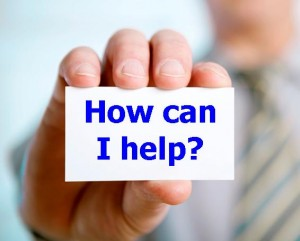
\includegraphics[width=6cm]{img/How-can-i-help.jpg}
\end{frame}

\begin{frame}{Identified needs}
We would like to build automated tools for the following tasks:
\begin{itemize}
\item Visualize system state
\item Identify anomalies
\item Predict Remaining Useful Life (RUL) / Time To Failure (TTF)
\item Predict failure occurrence or probability at a given horizon
\end{itemize}
~\\
Traditionaly, all this is based on user expertise.\\
Let's take a data-driven approach.
\end{frame}

\begin{frame}{Data analysis workflow for Predictive Maintenance}
\begin{enumerate}
\item<1-> Collect
\item<2-> Analyse
\item<3-> Predict
\item<4-> React
\end{enumerate}
\begin{overlayarea}{10cm}{4cm}
\begin{block}{}
\only<1>{
\begin{itemize}
\item Sensors deployment
\item Historical data collection
\item Integrated storage and retrieval issues
\end{itemize}
}
\only<2>{
\begin{itemize}
\item data cleaning
\item feature selection / engineering
\item algorithm selection
\item parameters tuning
\end{itemize}
}
\only<3>{
\begin{itemize}
\item Deploy solution in your operational process
\item Make things usable
\end{itemize}
}
\only<4>{
\begin{itemize}
\item Improve your maintenance decisions
\end{itemize}
}
\only<5>{
Need to automate as many steps as possible in this workflow\\
\hspace{2cm}$\rightarrow$ data-driven approaches\\
\hspace{2cm}$\rightarrow$ Machine Learning for step 2 (and 3)
}
\end{block}
\end{overlayarea}
\end{frame}

\begin{frame}{A word on data quality}
\begin{itemize}
\item amount of data: data is often scarce
\item noise, errors, missing data, outdated data: reliability
\item high-dimensional data
\item class imbalance
\item heterogeneous data (scalars, booleans, time series, images, text, \ldots)
\end{itemize}
All these will influence your choice of Machine Learning solutions
\end{frame}

\begin{frame}{Machine Learning}
\centering
Machines that learn?\\
Let's try to give a general definition.\\
~\\
\visible<2>{Machine learning is a field of computer science that gives computer systems the ability to ``learn'' (i.e. progressively improve performance on a specific task) with data, without being explicitly programmed.}
\end{frame}

\begin{frame}{ML examples}
Examples
\end{frame}

\begin{frame}{ML tasks}
%% ML tasks: Sup / unsup / RL
%% Data: (x,y) / x / transitions
%% Purpose: mimic a function / find structural patterns in data / optimal control
%% Subfields: classif, regr / dim reduction, clustering / -
%% Names of algorithms:

Software:
\begin{itemize}
\item Many free libraries: scikit-learn, tensorflow, caffe, \ldots
\item Commercial embedded solutions (more or less specialized): Matlab, IBM, emaint, Microsoft, \ldots
\end{itemize}
\end{frame}

\begin{frame}{Evaluation}
Evaluating ML methods?
\begin{itemize}
\item Regression: RMSE, margin \ldots
\item Classification: Misclass rate, TP, FP, cross entropy, ROC\ldots
\item Clustering: similarity scores
\end{itemize}
\end{frame}

\begin{frame}{Relating PM and ML}

\end{frame}

\begin{frame}{Let's finish with a focus on a practical use-case}

\end{frame}

\end{document}
